\documentclass[tikz,border=6pt]{standalone}
\usetikzlibrary{decorations.pathmorphing}

\definecolor{qmcroot}{RGB}{86,64,48}
\definecolor{qmctrunk}{RGB}{112,73,38}
\definecolor{qmcbranch}{RGB}{94,72,45}
\definecolor{qmcleaf}{RGB}{72,128,78}
\definecolor{qmcfruit}{RGB}{148,0,24}
\definecolor{qmcsoft}{RGB}{238,241,232}

\tikzset{
	root/.style={draw=qmcroot, line width=8pt, line cap=round},
	trunk/.style={draw=qmctrunk, line width=26pt, line cap=round},
	limb/.style={draw=qmcbranch, line width=14pt, line cap=round},
	branch/.style={draw=qmcbranch, line width=8pt, line cap=round},
	twig/.style={draw=qmcbranch, line width=4pt, line cap=round},
	leaf/.style={circle, fill=qmcleaf!85, draw=qmcleaf!45!black, inner sep=2.3pt},
	fruit/.style={circle, fill=qmcfruit, draw=qmcfruit!45!black, inner sep=3pt},
	biglabel/.style={font=\sffamily\bfseries\Large, align=center, text=black},
	smalllabel/.style={font=\sffamily\bfseries\small, align=center, text=black}
}

\begin{document}
	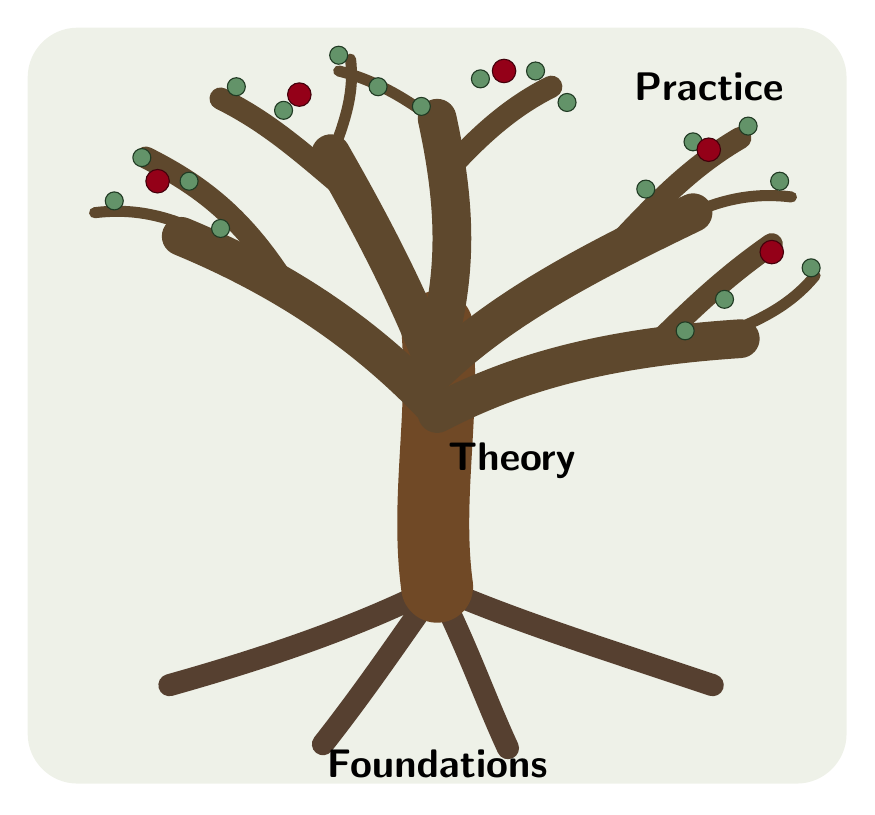
\begin{tikzpicture}[x=1cm,y=1cm]
		
		\fill[qmcsoft, rounded corners=18pt] (-5.2,-2.5) rectangle (5.2,7.1);
		
		\draw[root] (0,0) .. controls (-0.8,-0.4) and (-1.8,-0.8) .. (-3.4,-1.25);
		\draw[root] (0,0) .. controls (-0.5,-0.7) and (-0.9,-1.3) .. (-1.45,-2.0);
		\draw[root] (0,0) .. controls (0.4,-0.8) and (0.6,-1.4) .. (0.9,-2.05);
		\draw[root] (0,0) .. controls (0.9,-0.4) and (2.0,-0.75) .. (3.5,-1.25);
		
		\draw[trunk] (0,0) .. controls (-0.15,1.1) and (0.1,2.2) .. (0,3.3);
		
		\draw[limb] (0,2.25) .. controls (-0.8,3.1) and (-1.8,3.85) .. (-3.25,4.45);
		\draw[limb] (0,2.75) .. controls (-0.35,3.65) and (-0.75,4.45) .. (-1.35,5.5);
		\draw[limb] (0,3.05) .. controls (0.25,4.0) and (0.25,4.8) .. (0.0,5.95);
		\draw[limb] (0,2.75) .. controls (0.85,3.55) and (1.9,4.1) .. (3.25,4.75);
		\draw[limb] (0,2.2) .. controls (1.15,2.8) and (2.35,3.05) .. (3.85,3.15);
		
		\draw[branch] (-2.0,3.95) .. controls (-2.5,4.7) and (-3.0,5.1) .. (-3.7,5.45);
		\draw[branch] (-1.05,4.95) .. controls (-1.75,5.55) and (-2.15,5.9) .. (-2.75,6.2);
		\draw[branch] (0.1,5.25) .. controls (0.55,5.75) and (0.95,6.1) .. (1.45,6.35);
		\draw[branch] (2.2,4.25) .. controls (2.8,4.9) and (3.25,5.35) .. (3.85,5.7);
		\draw[branch] (2.75,3.05) .. controls (3.35,3.65) and (3.75,4.0) .. (4.25,4.35);
		
		\draw[twig] (-3.1,4.55) .. controls (-3.55,4.75) and (-3.95,4.8) .. (-4.35,4.75);
		\draw[twig] (-1.35,5.45) .. controls (-1.15,5.95) and (-1.05,6.3) .. (-1.1,6.7);
		\draw[twig] (0.0,5.9) .. controls (-0.45,6.25) and (-0.85,6.45) .. (-1.25,6.55);
		\draw[twig] (3.25,4.75) .. controls (3.7,4.95) and (4.1,5.0) .. (4.5,4.95);
		\draw[twig] (3.75,3.25) .. controls (4.25,3.45) and (4.55,3.65) .. (4.8,3.95);
		
		\foreach \p in {
			(-4.1,4.9),(-3.75,5.45),(-3.15,5.15),(-2.75,4.55),
			(-2.55,6.35),(-1.95,6.05),(-1.25,6.75),(-0.75,6.35),
			(-0.2,6.1),(0.55,6.45),(1.25,6.55),(1.65,6.15),
			(2.65,5.05),(3.25,5.65),(3.95,5.85),(4.35,5.15),
			(3.65,3.65),(4.25,4.25),(4.75,4.05),(3.15,3.25)
		}
		\node[leaf] at \p {};
		
		\node[fruit] at (-3.55,5.15) {};
		\node[fruit] at (-1.75,6.25) {};
		\node[fruit] at (0.85,6.55) {};
		\node[fruit] at (3.45,5.55) {};
		\node[fruit] at (4.25,4.25) {};
		
		\node[biglabel] at (0,-2.25) {Foundations};
		\node[biglabel] at (0.95,1.6) {Theory};
		\node[biglabel] at (3.45,6.35) {Practice};
		
	\end{tikzpicture}
\end{document}